% !TeX spellcheck = en_US
\chapter{Control as Inference}

\begin{itemize}
	\item \textit{Inference} means the process of inferring something, or a conclusion reached on the basis of evidence and reasoning.	
	\item \textit{Probabilistic inference} is the task of deriving the \ac{prob} of one or more random variables taking a specific value or set of values.
	\item \textit{Variational inference} lets us approximate a high-dimensional Bayesian posterior with a simpler variational distribution by solving an optimization problem.
\end{itemize}

\section{Probabilistic Graphical Model}
\label{sec:probabilistic-graphical-model}
Good behavior most of the time has minor mistakes here and there, though overall it is optimal. Thus, good behavior is rather suboptimal. Traditional optimal control doesn't not consider stochastic suboptimal behaviors like that.

\begin{itemize}
	\item Traditional probabilistic model of optimal control
	\begin{align*}
		&\textbf{a}_1, \dots, \textbf{a}_T = \underset{\textbf{a}_1, \dots, \textbf{a}_T}{\arg\max} \sum_{t=1}^T r(\textbf{s}_t, \textbf{a}_t)\\
		&\textbf{s}_{t+1} = f(\textbf{s}_t, \textbf{a}_t)
	\end{align*}	
	\item Probabilistic graphical model: $\mathcal{O}_t$ as the optimality variable
	\begin{align}
		p(\textbf{s}_{1:T}, \textbf{a}_{1:T}) &= p(\tau)\\
		p(\mathcal{O}| \textbf{s}_t, \textbf{a}_t) &= \exp (r(\textbf{s}_t, \textbf{a}_t))\\
		p(\tau | \mathcal{O}_{1:T}) &= \frac{p(\tau, \mathcal{O}_{1:T})}{p(\mathcal{O}_{1:T})}\\
		&\propto p(\tau) \prod_t \exp (r(\textbf{s}_t, \textbf{a}_t)) = p(\tau) \exp \left( \sum_t r(\textbf{s}_t, \textbf{a}_t) \right)
	\end{align}
	\begin{center}
		\begin{tikzpicture}[roundnode/.style={circle, draw=black!60, very thick, minimum size=7mm}]
			\node[roundnode](s1){$\textbf{s}_1$};
			\node[roundnode](s2)[right=3cm of s1]{$\textbf{s}_2$};	
			\node[roundnode](s3)[right=3cm of s2]{$\textbf{s}_3$};
			\node[roundnode](a1)[above right=1cm and 0.2cm of s1]{$\textbf{a}_1$};
			\node[roundnode](a2)[above right=1cm and 0.2cm of s2]{$\textbf{a}_2$};
			\node[roundnode](a3)[above right=1cm and 0.2cm of s3]{$\textbf{a}_3$};
			\node[roundnode, fill=gray](o1)[above left=.9cm and .5cm of a1]{$\mathcal{O}_1$};
			\node[roundnode, fill=gray](o2)[above left=.9cm and .5cm of a2]{$\mathcal{O}_2$};
			\node[roundnode, fill=gray](o3)[above left=.9cm and .5cm of a3]{$\mathcal{O}_3$};
			\draw[-latex](s1.east) -- (s2.west) node[midway, below]{$p(\textbf{s'|s,a})$};
			\draw[-latex](s2.east) -- (s3.west);
			\draw[-latex](a1.south east) -- (s2.west);
			\draw[-latex](a2.south east) -- (s3.west);
			\draw[-latex](s1.north) -- (o1.south);
			\draw[-latex](s2.north) -- (o2.south);
			\draw[-latex](s3.north) -- (o3.south);
			\draw[-latex](a1.north west) -- (o1.south east);
			\draw[-latex](a2.north west) -- (o2.south east);
			\draw[-latex](a3.north west) -- (o3.south east);
			\draw[-latex](s3.east) -- (12,0);
			\draw[-latex](a3.south east) -- (12,0);
			\node at (13,0) {\LARGE \textbf{\dots}};
		\end{tikzpicture}
	\end{center}
\end{itemize}

\section{Control as Inference}
\label{sec:control-as-inference}

Here, \textit{inference} implies planning. To do inference, we compute the three following terms:
\begin{align*}
	&\beta_t (\textbf{s}_t, \textbf{a}_t) = p(\mathcal{O}_{t:T}| \textbf{s}_t, \textbf{a}_t) && -\text{backward messages}\\
	&p(\textbf{a}_t | \textbf{s}_t, \mathcal{O}_{1:T}) && -\text{policy}\\
	&\alpha_t(\textbf{s}_t) = p(\textbf{s}_t | \mathcal{O}_{1:t-1}) && -\text{forward messages}\\
\end{align*}

\subsection{Backward Messages Computation}
Backward messages $\beta_t (\textbf{s}_t, \textbf{a}_t) = p(\mathcal{O}_{t:T}| \textbf{s}_t, \textbf{a}_t)$ is the \ac{prob} of optimality from the current time step $t$ till the end $T$, given the current state. $\textbf{s}_t$ and action $\textbf{a}_t$.
\begin{align*}
	\beta_t (\textbf{s}_t, \textbf{a}_t) &= p(\mathcal{O}_{t:T}| \textbf{s}_t, \textbf{a}_t) && -\text{the state-action backward message}\\
	\beta_t (\textbf{s}_t) &= p(\mathcal{O}_{t:T}| \textbf{s}_t) && -\text{the state backward message}
\end{align*}

Given:
\begin{align*}
	&p(\mathcal{O}_t| \textbf{s}_t, \textbf{a}_t) \propto \exp (r(\textbf{s}_t, \textbf{a}_t)) && \text{\ac{prob} of current optimality given state and action}\\
	&p(\textbf{s}_{t+1} | \textbf{s}_t, \textbf{a}_t) && \text{transition \ac{prob}}
\end{align*}

Formulation:
\begin{align}
	\beta_t (\textbf{s}_t, \textbf{a}_t)
	&= p(\mathcal{O}_{t:T}| \textbf{s}_t, \textbf{a}_t)\\
	&= \int p(\mathcal{O}_{t:T}, \textbf{s}_{t+1}| \textbf{s}_t, \textbf{a}_t) d\textbf{s}_{t+1}\\
	&= \int p(\mathcal{O}_{t+1:T}| \textbf{s}_{t+1}, \textbf{s}_t, \textbf{a}_t) p(\textbf{s}_{t+1} | \textbf{s}_t, \textbf{a}_t) p(\mathcal{O}_t| \textbf{s}_t, \textbf{a}_t) d\textbf{s}_{t+1}\\
	&= \int p(\mathcal{O}_{t+1:T}| \textbf{s}_{t+1}) \underbrace{p(\textbf{s}_{t+1} | \textbf{s}_t, \textbf{a}_t)}_{\text{known}} \underbrace{p(\mathcal{O}_t| \textbf{s}_t, \textbf{a}_t)}_{\text{known}} d\textbf{s}_{t+1}\\
	&= p(\mathcal{O}_t| \textbf{s}_t, \textbf{a}_t) \int p(\mathcal{O}_{t+1:T}| \textbf{s}_{t+1}) p(\textbf{s}_{t+1} | \textbf{s}_t, \textbf{a}_t)  d\textbf{s}_{t+1}\\
	\Rightarrow \beta_t (\textbf{s}_t, \textbf{a}_t)
	&= p(\mathcal{O}_t| \textbf{s}_t, \textbf{a}_t) \mathbb{E}_{\textbf{s}_{t+1} \sim p(\textbf{s}_{t+1} | \textbf{s}_t, \textbf{a}_t)} \left[ \beta_{t+1}(\textbf{s}_{t+1}) \right]\\
	p(\mathcal{O}_{t+1:T}| \textbf{s}_{t+1})
	&= \int \underbrace{p(\mathcal{O}_{t+1:T} | \textbf{s}_{t+1}, \textbf{a}_{t+1})}_{\text{backward message } \beta_{t+1} (\textbf{s}_{t+1}, \textbf{a}_{t+1})} \underbrace{p(\textbf{a}_{t+1} | \textbf{s}_{t+1})}_{\text{action prior}} d\textbf{a}_{t+1}\\
	\Rightarrow \beta_t (\textbf{s}_t) &= \mathbb{E}_{\textbf{a}_t \sim p(\textbf{a}_t | \textbf{s}_t)} \left[ \beta_t (\textbf{s}_t, \textbf{a}_t) \right] \qquad \text{(assuming uniform action prior $p(\textbf{a}_t | \textbf{s}_t)$)}
\end{align}

Recursive algorithm:
\begin{align}
	&\beta_T(\textbf{s}_T, \textbf{a}_T) =  p(\mathcal{O}_T| \textbf{s}_T, \textbf{a}_T) = \exp (r(\textbf{s}_T, \textbf{a}_T))\\
	&\text{for }t = T-1 \rightarrow 1:\\
	&\quad\beta_t (\textbf{s}_t, \textbf{a}_t) = p(\mathcal{O}_t| \textbf{s}_t, \textbf{a}_t) \mathbb{E}_{\textbf{s}_{t+1} \sim p(\textbf{s}_{t+1} | \textbf{s}_t, \textbf{a}_t)} \left[ \beta_{t+1}(\textbf{s}_{t+1}) \right] \\
	&\quad\beta_t (\textbf{s}_t) = \mathbb{E}_{\textbf{a}_t \sim p(\textbf{a}_t | \textbf{s}_t)} \left[ \beta_t (\textbf{s}_t, \textbf{a}_t) \right]
\end{align}

\hlb{Further examination:}
\begin{align*}
	&\text{let}\; V_t(\textbf{s}_t) = \log \beta_t(\textbf{s}_t)\\
	&\text{let}\; Q_t(\textbf{s}_t, \textbf{a}_t) = \log \beta_t(\textbf{s}_t, \textbf{a}_t)\\
	&V_t(\textbf{s}_t) = \log \int \exp \big( Q_t(\textbf{s}_t, \textbf{a}_t) \big) d\textbf{a}_t\\
	&V_t(\textbf{s}_t) \rightarrow \underset{\textbf{a}_t}{\max} Q_t(\textbf{s}_t, \textbf{a}_t) \; \text{as $Q_t(\textbf{s}_t, \textbf{a}_t)$ gets bigger!} \Rightarrow \text{"soft max"}\\
	&Q_t(\textbf{s}_t, \textbf{a}_t) = r(\textbf{s}_t, \textbf{a}_t) + \log \mathbb{E} [\exp V_{t+1}(\textbf{s}_{t+1})]\\
	&Q_t(\textbf{s}_t, \textbf{a}_t) = r(\textbf{s}_t, \textbf{a}_t) + V_{t+1}(\textbf{s}_{t+1}) \quad \text{in case of deterministic transition}
\end{align*}
The above looks a lot like Bellman's equation $\Rightarrow$ $\log$ of $\beta_t$ is "Q-function-like"

\note Value functions are backward messages.

\subsection{The Action Prior}
Re-examine the action prior when computing the backward messages. Before, we assume it was uniform (as a constant to be ignored). If it's not uniform:

\begin{align}
	p(\mathcal{O}_{t+1:T}| \textbf{s}_{t+1}) &= \int \beta_{t+1} (\textbf{s}_{t+1}, \textbf{a}_{t+1}) p(\textbf{a}_{t+1} | \textbf{s}_{t+1}) d\textbf{a}_{t+1} = \beta_{t+1}(\textbf{s}_{t+1})\\
	\Rightarrow V(\textbf{s}_t) &= \log \int \exp \big( Q_t(\textbf{s}_t, \textbf{a}_t) + \log p(\textbf{a}_t | \textbf{s}_t) \big) d\textbf{a}_t = \log \beta_t(\textbf{s}_t) \\
	Q_t(\textbf{s}_t, \textbf{a}_t) &= r(\textbf{s}_t, \textbf{a}_t) + \log \mathbb{E} [\exp V_{t+1}(\textbf{s}_{t+1})] && \text{(before)}\\
	\widetilde{Q}_t(\textbf{s}_t, \textbf{a}_t) &= r(\textbf{s}_t, \textbf{a}_t) + \log p(\textbf{a}_t | \textbf{s}_t) + \log \mathbb{E} [\exp V_{t+1}(\textbf{s}_{t+1})] &&\text{(modified)}\\
	\Rightarrow V(\textbf{s}_t) &=  \log \int \exp \big( \widetilde{Q}_t(\textbf{s}_t, \textbf{a}_t)\big) d\textbf{a}_t
\end{align}
Thus, a simple modification to the reward will take account of the non-uniform action prior.\\
$\Rightarrow$ we can assume uniform action prior without loss of generality.

\subsection{Policy Computation}
\label{subsec:policy-computation}
The policy $p(\textbf{a}_t | \textbf{s}_t, \mathcal{O}_{1:T})$ is the current action \ac{prob} given the current state $\textbf{s}_t$ that the whole trajectory is optimal.

Given:
\begin{align*}
	&p(\mathcal{O}_t| \textbf{s}_t, \textbf{a}_t) \propto \exp (r(\textbf{s}_t, \textbf{a}_t)) && -\text{\ac{prob} of current optimality given state and action}\\
	&p(\textbf{s}_{t+1} | \textbf{s}_t, \textbf{a}_t) && -\text{transition \ac{prob}}\\
	&\beta_t (\textbf{s}_t, \textbf{a}_t) = p(\mathcal{O}_{t:T}| \textbf{s}_t, \textbf{a}_t) && -\text{backward messages}\\
	&\beta_t (\textbf{s}_t) = p(\mathcal{O}_{t:T}| \textbf{s}_t) && -\text{backward state messages}
\end{align*}

Formulation:
\begin{align}
	p(\textbf{a}_t | \textbf{s}_t, \mathcal{O}_{1:T})
	&= \pi(\textbf{a}_t | \textbf{s}_t) = p(\textbf{a}_t | \textbf{s}_t, \mathcal{O}_{t:T})\\
	&= \frac{p(\textbf{a}_t, \textbf{s}_t | \mathcal{O}_{t:T})}{p(\textbf{s}_t | \mathcal{O}_{t:T})}\\
	&= \frac{p(\mathcal{O}_{t:T} | \textbf{a}_t, \textbf{s}_t) p(\textbf{a}_t, \textbf{s}_t) / p(\mathcal{O}_{t:T})}{p(\mathcal{O}_{t:T} | \textbf{s}_t) p(\textbf{s}_t) / p(\mathcal{O}_{t:T})} \qquad\qquad\text{(Bayes rule)}\\
	&= \frac{p(\mathcal{O}_{t:T} | \textbf{a}_t, \textbf{s}_t)}{p(\mathcal{O}_{t:T} | \textbf{s}_t)} \frac{p(\textbf{a}_t, \textbf{s}_t)}{p(\textbf{s}_t)} = \frac{\beta_t (\textbf{s}_t, \textbf{a}_t)}{\beta_t (\textbf{s}_t)} p(\textbf{a}_t | \textbf{s}_t)\\
	\Rightarrow \pi(\textbf{a}_t | \textbf{s}_t) &= \frac{\beta_t (\textbf{s}_t, \textbf{a}_t)}{\beta_t (\textbf{s}_t)} \qquad\qquad \text{(assume uniform action prior $p(\textbf{a}_t | \textbf{s}_t)$=const)}
\end{align}

Recursive algorithm:
\begin{align}
	&\text{for }t = T-1 \rightarrow 1:\\
	&\quad Q_t(\textbf{s}_t, \textbf{a}_t) = r(\textbf{s}_t, \textbf{a}_t) + \log \mathbb{E} \left[ \exp ( V_{t+1}(\textbf{s}_{t+1}) ) \right]\\
	&\quad V_t(\textbf{s}_t) = \log \int \exp \big(Q_t(\textbf{s}_t, \textbf{a}_t) \big) d\textbf{a}_t
\end{align}

Policy computation with value functions:
\begin{align}
	\pi(\textbf{a}_t | \textbf{s}_t) &= \frac{\beta_t (\textbf{s}_t, \textbf{a}_t)}{\beta_t (\textbf{s}_t)} \quad \text{with}\;\begin{cases}
		V_t(\textbf{s}_t) = \log \beta_t (\textbf{s}_t)\\
		Q_t(\textbf{s}_t, \textbf{a}_t) = \log \beta_t (\textbf{s}_t, \textbf{a}_t)
	\end{cases}\\
	\Rightarrow \pi(\textbf{a}_t | \textbf{s}_t) &= \exp \big(Q_t(\textbf{s}_t, \textbf{a}_t) - V_t(\textbf{s}_t)\big) = \exp \big( A_t(\textbf{s}_t, \textbf{a}_t)\big)
\end{align}
$\Rightarrow$ Soft advantage function with temperature:
\begin{equation}
	\pi(\textbf{a}_t | \textbf{s}_t) = \exp \left(\frac{1}{\alpha} A_t(\textbf{s}_t, \textbf{a}_t)\right) \quad \begin{cases}
		\alpha \rightarrow 0:\; \text{more deterministic}\\
		\alpha \rightarrow 1:\; \text{classical inference framework}
\end{cases}
\end{equation}

\subsection{Forward Messages Computation}
The forward messages $\alpha_t(\textbf{s}_t) = p(\textbf{s}_t | \mathcal{O}_{1:t-1})$ is the \ac{prob} of the state $\textbf{s}_t$ given that all previous trajectory steps are so far optimal.

Given:
\begin{align*}
	&p(\mathcal{O}_t| \textbf{s}_t, \textbf{a}_t) \propto \exp (r(\textbf{s}_t, \textbf{a}_t)) && -\text{\ac{prob} of current optimality given state and action}\\
	&p(\textbf{s}_{t+1} | \textbf{s}_t, \textbf{a}_t) && -\text{transition \ac{prob}}\\
	&\alpha(\textbf{s}_1) = p(\textbf{s}_1) && -\text{usually known}
\end{align*}

Formulation:
\begin{align}
	\alpha(\textbf{s}_t) &= p(\textbf{s}_t | \mathcal{O}_{1:t-1})\\
	&= \int p(\textbf{s}_t, \textbf{s}_{t-1}, \textbf{a}_{t-1} | \mathcal{O}_{1:t-1}) d\textbf{s}_{t-1} d\textbf{a}_{t-1}\\
	&= \int p(\textbf{s}_t | \textbf{s}_{t-1}, \textbf{a}_{t-1}, \mathcal{O}_{1:t-1}) p(\textbf{a}_{t-1} |\textbf{s}_{t-1}, \mathcal{O}_{1:t-1}) p(\textbf{s}_{t-1} | \mathcal{O}_{1:t-1}) d\textbf{s}_{t-1} d\textbf{a}_{t-1} \\
	&= \int \underbrace{p(\textbf{s}_t | \textbf{s}_{t-1}, \textbf{a}_{t-1})}_{\text{given}} p(\textbf{a}_{t-1} |\textbf{s}_{t-1}, \mathcal{O}_{t-1}) p(\textbf{s}_{t-1} | \mathcal{O}_{1:t-1}) d\textbf{s}_{t-1} d\textbf{a}_{t-1}
\end{align}
\begin{align}
	p(\textbf{a}_{t-1} |\textbf{s}_{t-1}, \mathcal{O}_{t-1}) p(\textbf{s}_{t-1} | \mathcal{O}_{1:t-1}) &= \frac{p(\mathcal{O}_{t-1} | \textbf{s}_{t-1}, \textbf{a}_{t-1}) p(\textbf{a}_{t-1} | \textbf{s}_{t-1})}{p(\mathcal{O}_{t-1} | \textbf{s}_{t-1})} \frac{p(\mathcal{O}_{t-1} | \textbf{s}_{t-1}) p(\textbf{s}_{t-1} | \mathcal{O}_{1:t-2})}{p(\mathcal{O}_{t-1} | \mathcal{O}_{1:t-2})}\\
	&= \underbrace{p(\mathcal{O}_{t-1} | \textbf{s}_{t-1}, \textbf{a}_{t-1})}_{\text{given}} \underbrace{p(\textbf{a}_{t-1} | \textbf{s}_{t-1})}_{\text{action prior}} \frac{\overbrace{p(\textbf{s}_{t-1} | \mathcal{O}_{1:t-2})}^{\textstyle \alpha_{t-1}(\textbf{s}_{t-1})}}{p(\mathcal{O}_{t-1} | \mathcal{O}_{1:t-2})}
\end{align}

The state marginal:
\begin{align}
	p(\textbf{s}_t | \mathcal{O}_{1:T}) =& \frac{p(\textbf{s}_t, \mathcal{O}_{1:T}) }{p(\mathcal{O}_{1:T})} = \frac{\overbrace{p(\mathcal{O}_{t:T} | \textbf{s}_t)}^ {\textstyle \beta_t(\textbf{s}_t)} p(\textbf{s}_t, \mathcal{O}_{1:t-1} )} {p(\mathcal{O}_{1:T})}\\
	& \propto \beta_t(\textbf{s}_t)	\underbrace{p(\textbf{s}_t | \mathcal{O}_{1:t-1})}_{\textstyle \alpha_t(\textbf{s}_t)} p(\mathcal{O}_{1:t-1}) \propto \beta_t(\textbf{s}_t) \alpha_t(\textbf{s}_t)
\end{align}

\subsection{Forward / Backward Message Intersection}
\begin{figure}[hbt!]
	\centering
	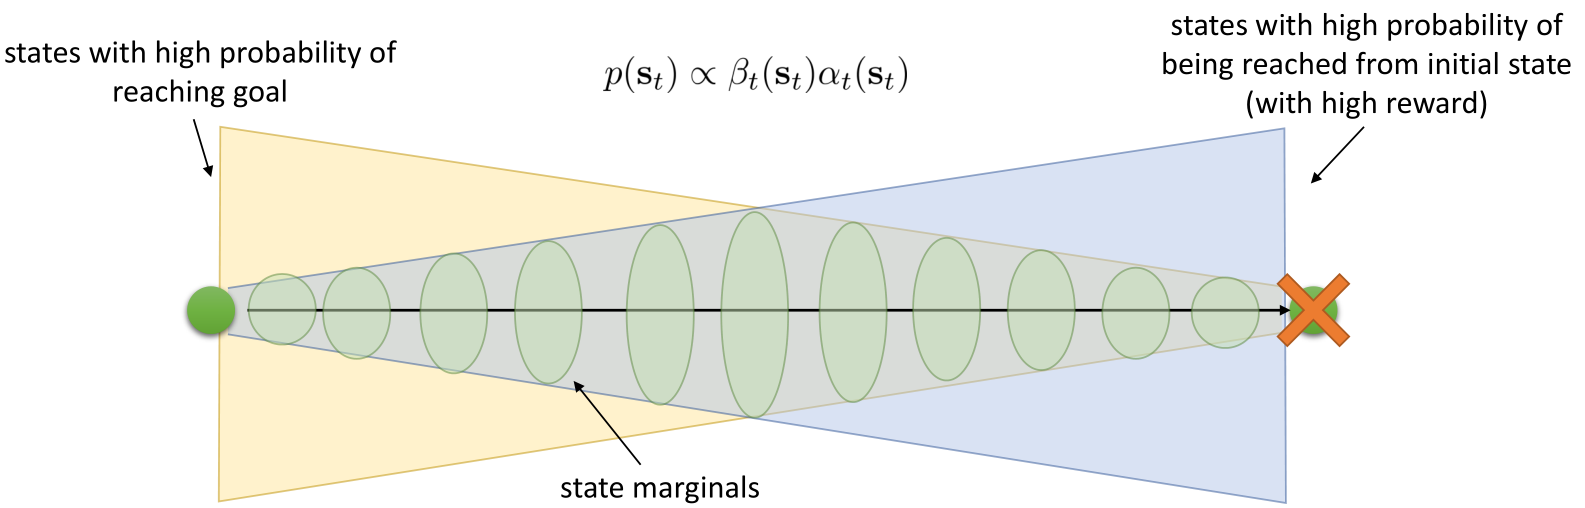
\includegraphics[width=.7\textwidth]{forward-backward-message-intersection.png}
	\caption{The intersection of backward and forward messages as state marginal (\href{http://rail.eecs.berkeley.edu/deeprlcourse/static/slides/lec-19.pdf}{UC Berkeley}).}
\end{figure}

\section{Control as Variational Inference}
\subsection{Optimism Problem}
The problem is due to the fact that given that you obtained high reward, the transition probability changes $p(\textbf{s}_{t+1} | \textbf{s}_t, \textbf{a}_t, \mathcal{O}_{1:T}) \neq p(\textbf{s}_{t+1} | \textbf{s}_t, \textbf{a}_t)$.
\begin{equation}
	Q_t(\textbf{s}_t, \textbf{a}_t) = r(\textbf{s}_t, \textbf{a}_t) + \underbrace{\log \mathbb{E} \left[ \exp ( V_{t+1}(\textbf{s}_{t+1}) ) \right]}_{\textstyle \text{"optimistic" transition}}
\end{equation}
Unlike in classic \ac{MDP}, the $\log$ of expectation of $\exp$ value function is overly optimistic, in the sense that a single large reward will overwhelm other values, while the average reward in expectation is low.

\hlb{Problem:} given that you obtained high reward, what was your action probability, \textit{given that your transition probability did not change?}

\hlb{Idea:} find a distribution $q(\textbf{s}_{1:T}, \textbf{a}_{1:T}) \approx p(\textbf{s}_{1:T}, \textbf{a}_{1:T} | \mathcal{O}_{1:T})$ but has dynamics $p(\textbf{s}_{t+1} | \textbf{s}_t, \textbf{a}_t)$

\subsection{Control via Variational Inference}
\begin{itemize}
	\item Let $\textbf{x} = \mathcal{O}_{1:T}$ and $z=(\textbf{s}_{1:T}, \textbf{a}_{1:T})$\\
	$\Rightarrow$ find $q(\textbf{z}) \approx p(\textbf{z}|\textbf{x})$
	\item Let $q(\textbf{z}) = q(\textbf{s}_{1:T}, \textbf{a}_{1:T}) = p(\textbf{s}_1) \prod_t p(\textbf{s}_{t+1} | \textbf{s}_t, \textbf{a}_t) q(\textbf{a}_t | \textbf{s}_t)$
\end{itemize}

The variational lower bound: $\log p(\textbf{x}) \geq \mathbb{E}_{\textbf{z} \sim q(\textbf{z})} [\log p(\textbf{x,z}) - \log q(\textbf{z})]$ (\href{AI_notes.pdf}{AI notes})
\begin{align*}	
	\Rightarrow \log p(\mathcal{O}_{1:T}) \geq \mathbb{E}_{(\textbf{s}_{1:T}, \textbf{a}_{1:T}) \sim q} \Bigg[ &\log p(\textbf{s}_1) + \sum_{t=1}^T \log p(\textbf{s}_{t+1} | \textbf{s}_t, \textbf{a}_t) + \sum_{t=1}^T \log p(\mathcal{O}_t | \textbf{s}_t, \textbf{a}_t) \\
	-&\log p(\textbf{s}_1) - \sum_{t=1}^T \log p(\textbf{s}_{t+1} | \textbf{s}_t, \textbf{a}_t) - \sum_{t=1}^T \log q(\textbf{a}_t | \textbf{s}_t) \Bigg]\\
	= \mathbb{E}_{(\textbf{s}_{1:T}, \textbf{a}_{1:T}) \sim q} \Bigg[ & \sum_t r(\textbf{s}_t, \textbf{a}_t) - \log q(\textbf{a}_t | \textbf{s}_t) \Bigg]\\
	= \sum_t \mathbb{E}_{(\textbf{s}_t, \textbf{a}_t) \sim q}  [r&(\textbf{s}_t, \textbf{a}_t) + \mathcal{H}(q(\textbf{a}_t | \textbf{s}_t))]
\end{align*}
$\Rightarrow$ This objective is the \ac{RL} objective, plus the action entropy. The additional action entropy term will give us more sub-optimal actions.

\hlb{Optimization with dynamic programming:}\\
- Base case: solve for the last time step $q(\textbf{a}_T | \textbf{s}_T)$
\begin{align*}
	q(\textbf{a}_T | \textbf{s}_T) &= \arg\max \mathbb{E}_{\textbf{s}_T \sim q (\textbf{s}_T)} \big[ \mathbb{E}_{\textbf{a}_T \sim q (\textbf{a}_T | \textbf{s}_T)} [r(\textbf{s}_T, \textbf{a}_T)] + \mathcal{H}(q(\textbf{a}_T | \textbf{s}_T)) \big]\\
	&= \arg\max \mathbb{E}_{\textbf{s}_T \sim q (\textbf{s}_T)} \big[ \mathbb{E}_{\textbf{a}_T \sim q (\textbf{a}_T | \textbf{s}_T)} [r(\textbf{s}_T, \textbf{a}_T) - \log q(\textbf{a}_T | \textbf{s}_T)] \big]
\end{align*}
Taking the derivative will result in: $q(\textbf{a}_T | \textbf{s}_T) \propto \exp(r(\textbf{s}_T, \textbf{a}_T))$
\begin{align}
	&q(\textbf{a}_T | \textbf{s}_T) = \frac{\exp (r(\textbf{s}_T, \textbf{a}_T))}{\int \exp(r(\textbf{s}_T, \textbf{a})) d\textbf{a}} = \exp \big( Q(\textbf{s}_T, \textbf{a}_T) - V(\textbf{s}_T) \big)\\
	&V(\textbf{s}_T) = \log \int \exp (Q(\textbf{s}_T, \textbf{a}_T)) d\textbf{a}_T\\
	\Rightarrow &\mathbb{E}_{\textbf{s}_T \sim q (\textbf{s}_T)} \big[ \mathbb{E}_{\textbf{a}_T \sim q (\textbf{a}_T | \textbf{s}_T)} [r(\textbf{s}_T, \textbf{a}_T) - \log q(\textbf{a}_T | \textbf{s}_T)] \big] = \mathbb{E}_{\textbf{s}_T \sim q (\textbf{s}_T)} \big[ \mathbb{E}_{\textbf{a}_T \sim q (\textbf{a}_T | \textbf{s}_T)} [V(\textbf{s}_T)] \big]
\end{align}
- At any time step: 
\begin{align*}
	Q_t(\textbf{s}_t, \textbf{a}_t) &= r(\textbf{s}_t, \textbf{a}_t) + \mathbb{E}[V_{t+1}(\textbf{s}_{t+1})] \qquad\text{(\textit{regular }Bellman backup - \textbf{not} optimistic)}\\
	q(\textbf{a}_t | \textbf{s}_t) &= \arg\max \mathbb{E}_{\textbf{s}_t \sim q (\textbf{s}_t)} \big[ \mathbb{E}_{\textbf{a}_t \sim q (\textbf{a}_t | \textbf{s}_t)} [r(\textbf{s}_t, \textbf{a}_t) + \mathbb{E}_{\textbf{s}_{t+1} \sim p(\textbf{s}_{t+1} | \textbf{s}_t, \textbf{a}_t)}[V(\textbf{s}_{t+1})]] + \mathcal{H}(q(\textbf{a}_t | \textbf{s}_t)) \big]\\
	&= \arg\max \mathbb{E}_{\textbf{s}_t \sim q (\textbf{s}_t)} \big[ \mathbb{E}_{\textbf{a}_t \sim q (\textbf{a}_t | \textbf{s}_t)} [Q(\textbf{s}_t, \textbf{a}_t)] + \mathcal{H}(q(\textbf{a}_t | \textbf{s}_t)) \big]\\
	&= \arg\max \mathbb{E}_{\textbf{s}_t \sim q (\textbf{s}_t)} \big[ \mathbb{E}_{\textbf{a}_t \sim q (\textbf{a}_t | \textbf{s}_t)} [Q(\textbf{s}_t, \textbf{a}_t) - \log q(\textbf{a}_t | \textbf{s}_t) ]\big]\\
	&\text{optimized when:}\; q(\textbf{a}_t | \textbf{s}_t) \propto \exp(Q_t(\textbf{s}_t, \textbf{a}_t))\\
	&V_t(\textbf{s}_t) = \log \int \exp(Q_t(\textbf{s}_t, \textbf{a}_t)) d\textbf{a}_t\\
	&q(\textbf{a}_t | \textbf{s}_t) = \exp \big( Q_t(\textbf{s}_t, \textbf{a}_t) - V_t(\textbf{s}_t) \big)
\end{align*}

Now we have a dynamic programming \ac{algor} for backward pass, \ac{aka} \textit{soft} value iteration \ac{algor}, which is similar to value iteration \ac{algor}:
\begin{align*}
	&\text{for}\; t=T-1 \rightarrow 1:\\
	&\quad Q_t(\textbf{s}_t, \textbf{a}_t) = r(\textbf{s}_t, \textbf{a}_t) + \mathbb{E}[V_{t+1}(\textbf{s}_{t+1})]\\
	&\quad V_t(\textbf{s}_t) = \log \int \exp(Q_t(\textbf{s}_t, \textbf{a}_t)) d\textbf{a}_t
\end{align*}

\begin{multicols}{2}
	Value iteration \ac{algor} (\secref{sec:value-iteration})
	\begin{enumerate}
		\item \tikzmark{via1}set $Q(\textbf{s,a}) \leftarrow r(\textbf{s,a}) + \gamma \mathbb{E}[V(\textbf{s}')]$
		\item \tikzmark{via2}set $V(\textbf{s}) \leftarrow \max_a Q(\textbf{s,a})$
		\begin{tikzpicture}[overlay,remember picture]
			\draw[very thick, -latex]
			([xshift=-7mm,yshift=1mm]pic cs:via2) --++ (-.5,0) |-
			([xshift=-7mm,yshift=1mm]pic cs:via1);
		\end{tikzpicture}
	\end{enumerate}
	\textit{Soft} value iteration \ac{algor} \cite{levine2018reinforcement}
	\begin{enumerate}
		\item \tikzmark{svia1}set $Q(\textbf{s,a}) \leftarrow r(\textbf{s,a}) + \gamma \mathbb{E}[V(\textbf{s}')]$
		\item \tikzmark{svia2}set $V(\textbf{s}) \leftarrow {\color{red}\text{soft} \max}_a Q(\textbf{s,a})$
		\begin{tikzpicture}[overlay,remember picture]
			\draw[very thick, -latex]
			([xshift=-7mm,yshift=1mm]pic cs:svia2) --++ (-.5,0) |-
			([xshift=-7mm,yshift=1mm]pic cs:svia1);
		\end{tikzpicture}
	\end{enumerate}
\end{multicols}

Variants:
\begin{itemize}
	\item Discounted SOC: $Q_t(\textbf{s}_t, \textbf{a}_t) = r(\textbf{s}_t, \textbf{a}_t) + {\color{red}\gamma} \mathbb{E} [V_{t+1}(\textbf{s}_{t+1})]$
	\item Explicit temperature: $V_t(\textbf{s}_t) = {\color{red}\alpha} \log \int \exp({\color{red}\frac{1}{\alpha}}Q_t(\textbf{s}_t, \textbf{a}_t)) d\textbf{a}_t$
\end{itemize}

\section{RL Algorithms as Inference}
Benefits of soft optimality
\begin{itemize}
	\item Improve exploration and prevent entropy collapse
	\item Easier to specialize (finetune) policies for more specific tasks
	\item Principled approach to break ties
	\item Better robustness (due to wider coverage of states)
	\item Can reduce to hard optimality as reward magnitude increases
	\item Good model for modeling human behavior
\end{itemize}

\subsection{Soft Q-Learning}
Q-Learning with Soft Optimality simply changes to the soft $\max$:
\begin{itemize}
	\item Standard Q-learning (\secref{sec:dql}):
	\begin{align*}
		&\phi \leftarrow \phi + \alpha \nabla_\phi Q_\phi(\textbf{s,a}) \big( r(\textbf{s,a}) + \gamma V(\textbf{s}') - Q_\phi(\textbf{s,a}) \big)\\
		&V(\textbf{s}') = \max_{\textbf{a}'} Q_\phi(\textbf{s}', \textbf{a}') && \text{(target value)}
	\end{align*}
	\item Soft Q-learning:
	\begin{align*}
		&\phi \leftarrow \phi + \alpha \nabla_\phi Q_\phi(\textbf{s,a}) \big( r(\textbf{s,a}) + \gamma V(\textbf{s}') - Q_\phi(\textbf{s,a}) \big) \\
		&V(\textbf{s}') = {\color{red}\text{soft} \max}_{\textbf{a}'} Q_\phi(\textbf{s}', \textbf{a}') = \log \int \exp \big( Q_\phi(\textbf{s}', \textbf{a}')\big) d\textbf{a}' && \text{(target value)}\\
		&\pi(\textbf{a}|\textbf{s}) = \exp \big( Q_\phi(\textbf{s,a}) - V(\textbf{s}) \big) = \exp \big(A_\phi(\textbf{s,a})\big)
	\end{align*}
	\begin{enumerate}
		\item \tikzmark{sql1}Take some action $\textbf{a}_i$ and observe $(\textbf{s}_i, \textbf{a}_i, \textbf{s}_i', r_i)$, add it to $\mathcal{R}$
		\item Sample mini-batch $\{(\textbf{s}_j, \textbf{a}_j, \textbf{s}_j', r_j) \}$ from $\mathcal{R}$ uniformly
		\item Compute $y_j = r_j + \gamma {\color{red}\text{soft} \max}_{\textbf{a}_j'} Q_{\phi'}(\textbf{s}_j', \textbf{a}_j')$ using \textit{target} network $Q_{\phi'}$
		\item $\phi \leftarrow \phi - \alpha \sum_j \frac{dQ_\phi}{d\phi}(\textbf{s}_j, \textbf{a}_j) \left( Q_{\phi}(\textbf{s}_j, \textbf{a}_j) - y_j \right)$
		\item \tikzmark{sql5}Update $\phi'$: copy $\phi$ every $N$ steps, or Polyak average $\phi' \leftarrow \tau \phi' + (1-\tau) \phi$
		\begin{tikzpicture}[overlay,remember picture]
			\draw[very thick, -latex]
			([xshift=-7mm,yshift=1mm]pic cs:sql5) --++ (-.5,0) |-
			([xshift=-7mm,yshift=1mm]pic cs:sql1);
		\end{tikzpicture}
	\end{enumerate}
\end{itemize}

\subsection{Entropy Regularized Policy Gradient}
Policy gradient with soft optimality:\\
$\pi(\textbf{a}|\textbf{s}) = \exp \big( Q_\phi(\textbf{s,a}) - V(\textbf{s}) \big)$ optimizes $J(\theta) = \sum_t \mathbb{E}_{\pi(\textbf{s}_t, \textbf{a}_t)} [r(\textbf{s}_t, \textbf{a}_t)] + \mathbb{E}_{\pi(\textbf{s}_t)} [\mathcal{H}(\pi(\textbf{a}_t | \textbf{s}_t))]$

\hlb{Intuition:}
\begin{align*}
	&\pi(\textbf{a}|\textbf{s}) \propto \exp ( Q_\phi(\textbf{s,a})) \;\text{when $\pi$ minimizes}\; D_{KL} \left( \pi(\textbf{a}|\textbf{s}) \Big|\Big| \frac{1}{Z} \exp (Q(\textbf{s,a}))\right) \\
	&D_{KL} \left( \pi(\textbf{a}|\textbf{s}) \Big|\Big| \frac{1}{Z} \exp (Q(\textbf{s,a}))\right) = \mathbb{E}_{\pi(\textbf{a|s})} [Q(\textbf{s,a})] -\mathcal{H}(\pi)
\end{align*}

\subsection{Soft Policy Gradient vs Soft Q-Learning}
Soft policy gradient derivation:
\begin{align}
	J(\theta) &= \sum_t \mathbb{E}_{\pi(\textbf{s}_t, \textbf{a}_t)} [r(\textbf{s}_t, \textbf{a}_t)] + \mathbb{E}_{\pi(\textbf{s}_t)} [\mathcal{H}(\pi(\textbf{a}_t | \textbf{s}_t))]\\
	&= \sum_t \mathbb{E}_{\pi(\textbf{s}_t, \textbf{a}_t)} [r(\textbf{s}_t, \textbf{a}_t) - \log \pi(\textbf{a}_t | \textbf{s}_t)]\\
	\nabla_\theta J &= \nabla_\theta \left[ \sum_t \mathbb{E}_{\pi(\textbf{s}_t, \textbf{a}_t)} [r(\textbf{s}_t, \textbf{a}_t) - \log \pi(\textbf{a}_t | \textbf{s}_t)] \right]\\
	&\approx \frac{1}{N} \sum_i \sum_t \nabla_\theta \log \pi(\textbf{a}_t | \textbf{s}_t) \Bigg( r(\textbf{s}_t, \textbf{a}_t) + \Bigg(\underbrace{\sum_{t'=t+1}^T r(\textbf{s}_{t'}, \textbf{a}_{t'}) - \log \pi(\textbf{a}_{t'} | \textbf{s}_{t'})}_{\textstyle \approx Q(\textbf{s}_{t+1}, \textbf{a}_{t+1})} \Bigg) - \log\pi(\textbf{a}_t | \textbf{s}_t) - \cancel{1} \Bigg)
\end{align}
We can ignore the $-1$ in the end (baseline).

Recall $\pi(\textbf{a}_t | \textbf{s}_t) = \exp \big(Q_t(\textbf{s}_t, \textbf{a}_t) - V_t(\textbf{s}_t)\big)$ (\subsecref{subsec:policy-computation}): 
\begin{equation}
	\nabla_\theta J(\theta) \approx \frac{1}{N} \sum_i \sum_t \big( \nabla_\theta Q_t(\textbf{s}_t, \textbf{a}_t) - \nabla_\theta V_t(\textbf{s}_t) \big) \big( r(\textbf{s}_t, \textbf{a}_t) + Q(\textbf{s}_{t+1}, \textbf{a}_{t+1}) - Q_t(\textbf{s}_t, \textbf{a}_t) + \cancel{V(\textbf{s}_t)} \big)
\end{equation}
Because of the baseline properties, any state dependent baseline can be removed, thus, we can ignore the $V(\textbf{s}_t)$.

Soft Q-learning (gradient descent, instead of gradient ascent in policy gradient):
\begin{equation}
	\nabla_\theta J(\theta) \approx - \frac{1}{N} \sum_i \sum_t \nabla_\theta Q_t(\textbf{s}_t, \textbf{a}_t) \big( r(\textbf{s}_t, \textbf{a}_t) + \underset{\textbf{a}_{t+1}}{\text{soft}\max} Q(\textbf{s}_{t+1}, \textbf{a}_{t+1}) - Q_t(\textbf{s}_t, \textbf{a}_t)\big)
\end{equation}

\section{Soft Actor-Critic}
Algorithm overview \cite{haarnoja2018soft}:
\begin{enumerate}
	\item Q-function update to evaluate current policy: this converges to $Q^\pi$
	\begin{equation}
		Q(\textbf{s,a}) \leftarrow r(\textbf{s,a}) + \mathbb{E}_{\textbf{s}' \sim p_\textbf{s}, \textbf{a}' \sim \pi} [Q(\textbf{s}', \textbf{a}') {\color{red} - \log \pi(\textbf{a}' | \textbf{s}')}]
	\end{equation}
	\item Update policy with gradient of information projection
	\begin{equation}
		\pi_{new} = \underset{\pi'}{\arg\min} D_{KL} \left( \pi'(\cdot | \textbf{s}) \Big|\Big| \frac{1}{Z} \exp Q^{\pi_{old}}(\textbf{s}, \cdot) \right)
	\end{equation}
	In practice, only take one gradient step on this objective
	\item Interact with the world, collect more data
\end{enumerate}

\section{References}
\begin{itemize}
	\item \citeaus{todorov2006linearly}. Linearly-solvable Markov decision problems.
	\item \citeaus{todorov2008general}. General duality between optimal control and estimation.
	\item \citeaus{kappen2012optimal}. Optimal control as a graphical model inference problem.
	\item \citeaus{ziebart2010modeling}. Modeling interaction via the principle of maximum causal entropy.
	\item \citeaus{rawlik2012stochastic}. On stochastic optimal control and reinforcement learning by approximate inference.
	\item \citeausm{haarnoja2017reinforcement}. Reinforcement learning with deep energy-based policies.
	\item \citeausm{nachum2017bridging}. Bridging the gap between value and policy based reinforcement learning.
	\item \citeaus{schulman2017equivalence}. Equivalence between policy gradients and soft q-learning.
	\item \citeausm{haarnoja2018soft}. Soft actor-critic: Off-policy maximum entropy deep reinforcement learning with a stochastic actor.
	\item \citeaus{levine2018reinforcement}. Reinforcement learning and control as probabilistic inference: Tutorial and review.
\end{itemize}